\documentclass[a4paper,12pt]{article}

\usepackage[utf8]{inputenc}
\usepackage[german]{babel}
\usepackage{graphicx}
\usepackage{geometry}
\usepackage{graphicx}


\geometry{margin=2.5cm}

\title{Smarthome Project – Systemintegration}
\author{}
\date{}

\begin{document}

\maketitle

\section{Projektbeschreibung}

Bei unserem Smart-Home-Projekt geht es hauptsächlich um die Steuerung von Lampen eines Modellhauses über unterschiedliche Plattformen (Windows, Tablet – Android, VR – Android) mittels einer Industriesteuerung.

Die Lampen werden über Schalter in den einzelnen Räumen bedient und können ein- bzw. ausgeschaltet werden. Die Industriesteuerung übernimmt dabei die zentrale Rolle, da sie für die tatsächliche Ansteuerung der Hardware zuständig ist.

Unity dient zur Entwicklung der digitalen Varianten des Smart Homes. Zusätzlich existiert ein reales, gebautes Karton-Modell. Über die Ausgänge der Steuerung können Lampen geschaltet werden, wodurch das Licht sowohl im realen Modell als auch in Unity ein- und ausgeschaltet werden kann.

\section{Funktionsweise}

Unity dient in diesem Projekt als Entwicklungsumgebung für ein virtuelles Modell des Hauses, in dem ebenfalls Lampen integriert sind.

Wenn in Unity eine Lampe durch Betätigung eines Schalters eingeschaltet wird, wird ein Signal an die Industriesteuerung gesendet. Diese verarbeitet den Befehl und schaltet anschließend die Lampe auf allen Plattformen ein.

Zusätzlich wird der aktuelle Zustand der Lampe zurück an die Anwendungen übertragen. Dadurch ist auf allen Plattformen sichtbar, ob eine Lampe gerade ein- oder ausgeschaltet ist.

\section{Systemintegration}

Durch diese Kombination entsteht eine Verbindung zwischen virtueller Simulation und realer Steuerung.

Die Industriesteuerung sorgt für eine stabile und zuverlässige Kontrolle sowie für die Kommunikation mit der Hardware. Unity dient als Entwicklungsumgebung für die Anwendungen auf den unterschiedlichen Plattformen.

Die Apps übernehmen die Visualisierung und ermöglichen die Bedienung des digitalen Zwillings. Dadurch wird gezeigt, wie verschiedene Systeme und Plattformen miteinander interagieren können.

\section{Aufbau der Hardware}
\begin{figure}[h]
\centering
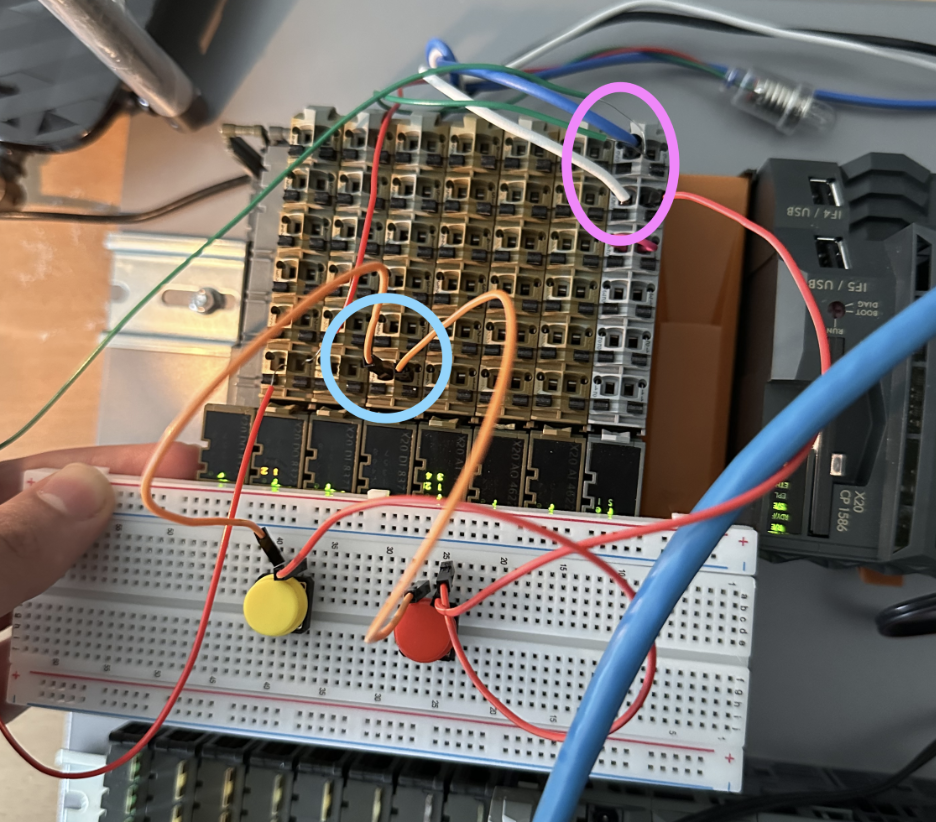
\includegraphics[width=0.6\textwidth]{image02.png}
\caption{Layout für Stromversorgung/Schalter}
\caption{Layout für Stromversorgung/Schalter}
\end{figure}


\subsection{Schritt 1: Stromversorgung}

Die Stromversorgung erfolgt über:
\begin{itemize}
    \item 24 V (weißes Kabel)
    \item GND (blaues Kabel)
\end{itemize}

Die Verkabelung erfolgt entsprechend des vorgegebenen Layouts.

\subsection{Schritt 2: Lichtschalter}

Die Lichtschalter werden auf einem Steckbrett montiert und mit der Industriesteuerung verbunden.

Dabei benötigen die Schalter:
\begin{itemize}
    \item eine Verbindung zur Stromversorgung
    \item eine Verbindung zu einem digitalen Eingang der Steuerung
\end{itemize}

\subsection{Schritt 3: Glühbirne}

Die Glühbirne benötigt zwei Verbindungen:
\begin{itemize}
    \item 24 V
    \item GND
\end{itemize}

Die 24 V werden über den Ausgang des Schalters geführt.

\section{Logik und Aufbau}

Die Steuerung basiert auf mehreren Eingängen:
\begin{itemize}
    \item Tablet
    \item Laptop
    \item VR-Headset
    \item Physischer Schalter (analog)
\end{itemize}

Zwischen den Eingängen und der Ausgabe wird eine logische ODER-Verknüpfung verwendet.

Zusätzlich erfolgt die Kommunikation über eine OPC-UA-Schnittstelle.

Am Ausgang befindet sich der Verbraucher, in diesem Fall eine Glühbirne. Dabei wird auf die positive Flanke des Signals geachtet, um das Schalten korrekt auszulösen.



\begin{figure}[h]
\centering
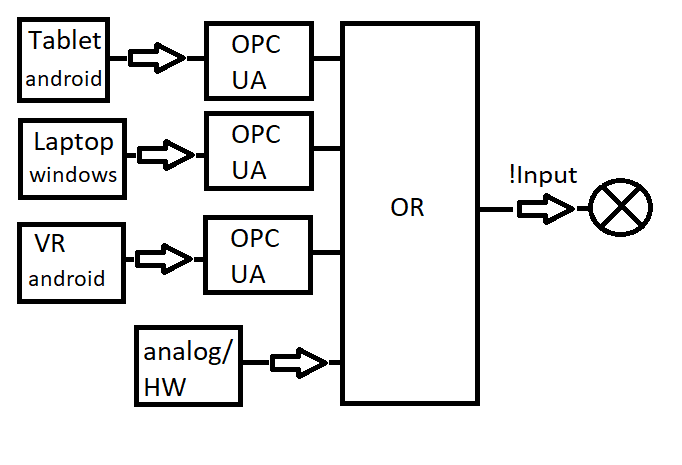
\includegraphics[width=0.6\textwidth]{image01.png}
\caption{Digitale Ein- und Ausgangskarte}

\end{figure}

\end{document}